\documentclass[times,numbers=noenddot]{itmo-student-thesis}

%% Опции пакета:
%% - specification - если есть, генерируется задание, иначе не генерируется
%% - annotation - если есть, генерируется аннотация, иначе не генерируется
%% - times - делает все шрифтом Times New Roman, собирается с помощью xelatex
%% - languages={...} - устанавливает перечень используемых языков. По умолчанию это {english,russian}.
%%                     Последний из языков определяет текст основного документа.

%% Делает запятую в формулах более интеллектуальной, например:
%% $1,5x$ будет читаться как полтора икса, а не один запятая пять иксов.
%% Однако если написать $1, 5x$, то все будет как прежде.
\usepackage{icomma}

%% Один из пакетов, позволяющий делать таблицы на всю ширину текста.
\usepackage{tabularx}

%% Данные пакеты необязательны к использованию в бакалаврских/магистерских
%% Они нужны для иллюстративных целей
%% Начало
\usepackage{tikz}
\usetikzlibrary{arrows}
\usepackage{filecontents}
\begin{filecontents}{bachelor-thesis.bib}
@online{ doerr-doerr-lambda-lambda-self-adjustment-arxiv,
    year        = {2015},
    title       = {Optimal Parameter Choices Through Self-Adjustment: Applying the 1/5-th Rule in
                   Discrete Settings},
    author      = {Benjamin Doerr and Carola Doerr},
    url         = {http://arxiv.org/abs/1504.03212},
    year        = {2015},
    langid      = {english}
}

@inproceedings{ example-english,
    year        = {2015},
    booktitle   = {Proceedings of IEEE Congress on Evolutionary Computation},
    author      = {Maxim Buzdalov and Anatoly Shalyto},
    title       = {Hard Test Generation for Augmenting Path Maximum Flow
                   Algorithms using Genetic Algorithms: Revisited},
    pages       = {2121-2128},
    langid      = {english}
}

@article{ example-russian,
    author      = {Максим Викторович Буздалов},
    title       = {Генерация тестов для олимпиадных задач по программированию
                   с использованием генетических алгоритмов},
    journal     = {Научно-технический вестник {СПбГУ} {ИТМО}},
    number      = {2(72)},
    year        = {2011},
    pages       = {72-77},
    langid      = {russian}
}

@article{ unrestricted-jump-evco,
    author      = {Maxim Buzdalov and Benjamin Doerr and Mikhail Kever},
    title       = {The Unrestricted Black-Box Complexity of Jump Functions},
    journal     = {Evolutionary Computation},
    year        = {2016},
    note        = {Accepted for publication},
    langid      = {english}
}

@book{ bellman,
    author      = {R. E. Bellman},
    title       = {Dynamic Programming},
    address     = {Princeton, NJ},
    publisher   = {Princeton University Press},
    numpages    = {342},
    pagetotal   = {342},
    year        = {1957},
    langid      = {english}
}
\end{filecontents}
%% Конец

%% Указываем файл с библиографией.
\addbibresource{bachelor-thesis.bib}

\begin{document}

\studygroup{К34212}
\title{Пример оформления ВКР бакалавра}
\author{Тельнов Федор Николаевич}{Тельнов Ф.Н.}
\supervisor{Самохин Никита Юрьевич}{Самохин Н.Ю.}
\curator{Федоров Дмитрий Алексеевич}{Федоров Д.А.}

\publishyear{2025}

%% Задание
%%% Техническое задание и исходные данные к работе
\technicalspec{Требуется разработать стилевой файл для системы \LaTeX, позволяющий оформлять бакалаврские работы и магистерские диссертации
	на кафедре компьютерных технологий Университета ИТМО. Стилевой файл должен генерировать титульную страницу пояснительной записки,
	задание, аннотацию и содержательную часть пояснительной записк. Первые три документа должны максимально близко соответствовать шаблонам документов,
	принятым в настоящий момент на кафедре, в то время как содержательная часть должна максимально близко соответствовать ГОСТ~7.0.11-2011
	на диссертацию.}

%%% Содержание выпускной квалификационной работы (перечень подлежащих разработке вопросов)
\plannedcontents{Пояснительная записка должна демонстрировать использование наиболее типичных конструкций, возникающих при составлении
	пояснительной записки (перечисления, рисунки, таблицы, листинги, псевдокод), при этом должна быть составлена так, что демонстрируется
	корректность работы стилевого файла. В частности, записка должна содержать не менее двух приложений (для демонстрации нумерации рисунков и таблиц
	по приложениям согласно ГОСТ) и не менее десяти элементов нумерованного перечисления первого уровня вложенности (для демонстрации корректности
	используемого при нумерации набора русских букв).}

%%% Исходные материалы и пособия
\plannedsources{\begin{enumerate}
		\item ГОСТ~7.0.11-2011 <<Диссертация и автореферат диссертации>>;
		\item С.М. Львовский. Набор и верстка в системе \LaTeX;
		\item предыдущий комплект стилевых файлов, использовавшийся на кафедре компьютерных технологий.
	\end{enumerate}}

%%% Цель исследования
\researchaim{Разработка удобного стилевого файла \LaTeX
	для бакалавров и магистров кафедры компьютерных технологий.}

%%% Задачи, решаемые в ВКР
\researchtargets{\begin{enumerate}
		\item обеспечение соответствия титульной страницы, задания и аннотации шаблонам, принятым в настоящее время на кафедре;
		\item обеспечение соответствия содержательной части пояснительной записки требованиям ГОСТ~7.0.11-2011 <<Диссертация и автореферат диссертации>>;
		\item обеспечение относительного удобства в использовании~--- указание данных об авторе и научном руководителе один раз и в одном месте, автоматический подсчет числа тех или иных источников.
	\end{enumerate}}

%%% Использование современных пакетов компьютерных программ и технологий
\addadvancedsoftware{Пакет \texttt{tabularx} для чуть более продвинутых таблиц}{\ref{sec:tables}, Приложения~\ref{sec:app:1}, \ref{sec:app:2}}
\addadvancedsoftware{Пакет \texttt{biblatex} и программное средство \texttt{biber}}{Список использованных источников}

%%% Краткая характеристика полученных результатов
\researchsummary{Получился, надо сказать, практически неплохой стилевик. В 2015--2018 годах
	его уже использовали некоторые бакалавры и магистры. Надеюсь на продолжение.}

%%% Гранты, полученные при выполнении работы
\researchfunding{Автор разрабатывал этот стилевик исключительно за свой счет и на
	добровольных началах. Однако значительная его часть была бы невозможна, если бы
	автор не написал в свое время кандидатскую диссертацию в \LaTeX,
	а также не отвечал за формирование кучи научно-технических отчетов по гранту,
	известному как <<5-в-100>>, что происходило при государственной финансовой поддержке
	ведущих университетов Российской Федерации (субсидия 074-U01).}

%%% Наличие публикаций и выступлений на конференциях по теме выпускной работы
\researchpublications{По теме этой работы я (к счастью!) ничего не публиковал.
	\begin{refsection}
		Однако покажу, как можно ссылаться на свои публикации из списка литературы:
		\nocite{example-english, example-russian}
		\printannobibliography
	\end{refsection}
}

%% Эта команда генерирует титульный лист и аннотацию.
\maketitle{Бакалавр}

%% Оглавление
\tableofcontents

\startshortenspage

API – Application Programming Interface

HTTP – HyperText Transfer Protocol

СУБД – Система управления базами данных

I/O - Input / Output

\startterminologypage

HTTP (HyperText Transfer Protocol) - протокол прикладного уровня, который используется для передачи данных в сети Интернет.
Он определяет правила и формат обмена данными между клиентом (например, веб-браузером) и сервером.

Акторные группы - группы пользователей, объединенных общими потребностями, проблемами, интересами и используемыми технологиями.
Отдельные акторные группы чаще всего действуют независимо, даже находясь в рамках одной организации.


%% Макрос для введения. Совместим со старым стилевиком.
\startprefacepage

В мире российского IT пользуется популярностью in-memory база данных Tarantool.
Ею пользуются как гиганты для реализации критичных к производительности сервисов, так и частные лица, заинтересованные в быстром проектировании отказоустойчивых и эффективных решений.
Долгое время приложения для Tarantool писались на языке Lua, однако в последнее время фокус сообщества начинает смещаться в сторону Rust.
Это объясняется неординарной безопасностью и эффективностью, которую предоставляет этот язык.
Компания Picodata, помимо создания собственного продукта, также занимается поддержкой и развитием Rust-экосистемы, фактически являясь единственным крупным ее мейнтейнером.

Lua - достаточно популярный выбор, когда речь заходит об интеграции бизнес-логики пользователя с существующим C API в рамках некоторого высокопроизводительного приложения.
Так, например, в рамках прокси и балансировщика нагрузки HAProxy можно реализовывать собственную логику маршрутизации запросов на языке Lua.
Обычно в рамках среды выполнения и диалекта языка в таком случае используется Lua JIT - версия интерпретатора Lua, разработанная с целью повышения производительности.
В рамках разработки СУБД Tarantool создатели пошли тем же маршрутом, и конечные пользователи получили возможность достаточно просто реализовывать бизнес-логику сложных систем обработки и хранения данных, при этом получая в среднем удовлетворяющий уровень производительности.
Однако, как показывает практика, системы в рамках СУБД Tarantool, написанные на языке Lua, зачастую не удовлетворяют SLA - Lua JIT дает временами потрясающую производительность, но имеет тенденцию к деградации.
Переходным периодом в жизни таких проектов можно считать интеграцию библиотек, написанных на других языках - например, для ускорения разбора JSON-запросов можно использовать SIMD-совместимую библиотеку на языке C++, добавив к ней API-обертку на языке Lua.

Компания Picodata решила пойти более кардинальным путем - в рамках собственного форка Tarantool и, в конечном итоге, в рамках СУБД Picodata, было решено постепенно избавить пользователя от языка Lua вовсе, предложив ему альтернативу для написания бизнес-приложений.
Целевым языком, на который был осуществлен переход, стал Rust: были созданы вспомогательные биндинги к C API СУБД Tarantool, утилиты для разработки.
Этот переход уже позволяет создавать высокопроизводительные системы полностью на современном языке программирования Rust - в результате SLA поддерживать стало проще, нет непредвиденных замедлений из-за Lua JIT.
Однако все еще остается проблема - множество частей СУБД Tarantool, которые внутренне используются СУБД Picodata, по-прежнему реализованы на языке Lua.
Например, к подобным компонентам относится реализация виртуального шардирования - библиотека vshard.
Наблюдая проблемы при эксплуатации, связанные с подобными компонентами, компания Picodata ведет инициативы по переписыванию этих частей на Rust.
Дополнительным преимуществом и упрощением в данном случае является постоянно расширяющаяся и активно поддерживаемая экосистема Rust-библиотек.

На данный момент приемом и обработкой входных данных от клиентов в рамках протокола HTTP занимается компонент “tarantool/http”, представляющий собой HTTP-сервер на языке Lua.
После получения данные в виде набора байт сначала разбираются и трансформируются в Lua-специфичный тип - таблицы.
Затем таблицы последовательно помещаются на стек и поглощаются с помощью биндингов на стороне Rust, переводятся в Rust-специфичные типы с помощью фреймворка “shors”, разработанного командой Picodata.
В результате каждый пользовательский запрос проходит этот путь: ценное время тратится на лишнюю трансформацию данных, что приводит к увеличению времени задержки запросов.
Если же старый компонент на Lua переписать на Rust, то данные сразу же будут доступны в нужной среде исполнения и в необходимом для конечного бизнес-приложения пользователя формате, что упрощает поддержку установленного SLA для сетевых приложений.
Кроме того, немаловажное преимущество - возможность использовать данный HTTP-сервер в рамках процесса работы самой СУБД Picodata.
Встроенных HTTP-эндпоинтов не так много, они нужны в основном для административных целей, но влияют на общую производительность кластера в виду однопоточной природы исполнительной(транзакционной) части СУБД Picodata.

Целью данной работы является разработка HTTP-сервера высокой производительности для СУБД Picodata.
Для начала будет проведен детальный анализ существующего решения - комбинации фреймворка “shors” на языке Rust и HTTP-сервера на Lua от Tarantool.
Будут выбраны акторные группы существующего решения, построена диаграмма прецедентов.
К новому продукту будут составлены функциональные и нефункциональные требования.
После будет представлено новое решение - полноценный HTTP-сервер на языке Rust для СУБД Picodata.
Конечное решение будет использоваться в качестве замены существующему в рамках пользовательских бизнес-приложений - в терминологии СУБД Picodata они называются плагинами, а также в рамках работы самого процесса Picodata.

В рамках данной работы были поставлены и достигнуты следующие цели:

\begin{enumerate}[label=\arabic*.]
	\item рассмотреть текущее решение, его преимущества и недостатки;
	\item изучить акторные группы текущего решения, построить диаграмму прецедентов;
	\item сформировать функциональные и нефункциональные требования для нового продукта;
	\item сформировать архитектуру будущего решения;
	\item сформировать первичную реализацию решения.
\end{enumerate}

%% Начало содержательной части.
\leftalignedtrue
\chapter{Исследование}
\leftalignedfalse

\section{Анализ существующего решения}\label{sec:analyze_existing}

Чтобы детально разобрать интеграцию старого HTTP-сервера на Lua со внутренними процессами СУБД Tarantool, необходимо рассмотреть архитектуру СУБД Tarantool по части реализации основного транзакционного потока и I/O.
Транзакционный поток Tarantool построен на принципе user-space потоков, которые по установленной терминологии документации Tarantool зовутся файберами.
Часто их также называют зелеными потоками или корутинами: главное их преимущество в легковесности - нет нужды в дорогостоящих переключениях контекста, в рамках одного системного потока уживаются множество параллельных “зеленых” потоков, выполняющихся по очереди.
Это позволяет оптимально утилизировать доступные ресурсы - так, весь процесс СУБД Tarantool использует всего несколько системных потоков.
У такого подхода есть и недостаток - нет принудительного переключения контекста.
Если при классической модели системных потоков некоторый поток процесса блокируется или неэффективно расходует ресурсы на некоторую долгую операцию, то он все равно будет переключен операционной системой.
Конечно, этот вопрос контролируется планировщиком ОС, но суть неизменна - не преэмптивное планирование позволяет принудительное переключение, что часто позволяет корректное выполнение даже при ошибке логики приложения.
При преэмптивном планировании, характерном в том числе для user-space потоков, такой возможности нет - если в рамках логики приложения по какой-то причине “зеленый” поток блокируется, он заблокирует выполнение остальных участников кооперативной многозадачности в рамках одного системного потока.
Особенно это критично, если используется единый системный поток - его блокировка будет означать остановку выполнения всех остальных частей приложения.
Это как раз случай Tarantool - большая часть пользовательской логики исполняется в одном транзакционном потоке.
Поэтому разработчики приложений на базе Tarantool стараются реализовать алгоритмы в файберах в итеративной манере - каждый файбер при переключении на него занимает немного процессорного времени, и снова засыпает, добровольно возвращая контроль над потоком планировщику.

В традиционной модели системных потоков в, например, синхронном сетевом вызове нет ничего плохого - при ожидании на сокете с использованием необходимого системного вызова, поток будет заблокирован и переключен планировщиком ОС, пока не будут получены данные.
В рамках же модели user-space потоков любой блокирующий вызов приведет к блокировке остальных участников.
Поэтому по части I/O-вызовов для user-space потоков разрабатывается собственная неблокирующая система, внутренне использующая функциональность встроенных I/O системных вызовов ОС.
В Tarantool пошли схожим путем: используется библиотека libev на языке C, предоставляющая реализацию event loop с интеграцией неблокирующих вызовов.
На рисунке 1.1 показана упрощенная схема работы транзакционного потока из документации Tarantool, построенного поверх libev - она демонстрирует чередование user-space потоков в рамках libev event loop, их обращение к арене - области памяти узла, отвечающей за непосредственное хранение данных.

\begin{figure}[!h]
	\caption*{Рисунок 1.1 - Схема работы event loop - файберы и арена}\label{fig1}
	\centering
	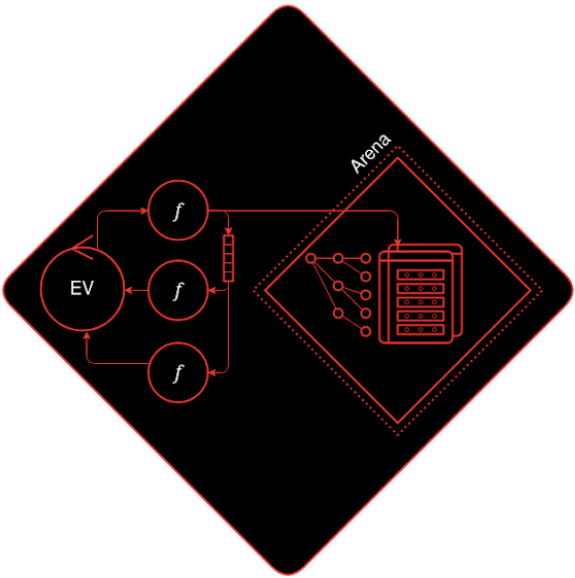
\includegraphics[scale=0.7]{tt_evloop}
\end{figure}


Указанная реализация предоставляет производительную однопоточную среду исполнения, хорошо подходит для реализации in-memory базы данных, однако требует аккуратного подхода к реализации любого I/O-взаимодействия.
Ключевая проблема - блокирующий вызов нарушает работу узла.
Неблокирующие методы работы с сокетами подходят, но схема ожидания их результата должна быть реализована через средства предоставляемой библиотеки, чтобы избежать лишнего опроса сокетов и пробуждения файберов.
Иными словами, транспортировку данных и их ожидание нужно делать через обертки над примитивами Tarantool и, в частности, CoIO.
Это накладывает мораторий на использование большинства готовых библиотек, например HTTP-клиента “reqwest” и HTTP-сервера “axum” из экосистемы Rust.

Одним из обходных путей является поднятие сторонней среды исполнения - еще одного набора потоков, и делегирование I/O работы на них.
Возникает проблема синхронизации двух сред исполнения - TX-потока Tarantool и сторонней среды.
Это зачастую приемлемое решение, и нередко используется в реальности, особенно когда необходимо использовать готовую библиотеку, предоставляющую обертку над HTTP-API некоторого сервиса.
В таких случаях используют библиотеку “tros”, реализующую удобный интерфейс для взаимодействия со сторонней средой исполнения.
У такого решения есть и недостатки: необходима синхронизация между потоками, передача данных между ними.
При интенсивности HTTP-трафика это приводит к нежелательному увеличению задержки обработки запроса.

Самым оптимальным по производительности выбором в итоге остается построение собственного фреймворка, используя предоставляемые Tarantool примитивы для неблокирующего I/O.
Так и построено существующее решение: реализован фреймворк HTTP на Lua, интегрирующийся с CoIO - системой неблокирующего I/O для Tarantool.
Поверх него уже для простоты реализации был построен Rust-фреймворк “shors”, помимо прочего предоставляющий удобное API и автоматическую генерацию OpenAPI-схемы.
В рамках этого перехода и происходит потеря ценного времени - Lua-фреймворк корректно интегрируются с CoIO, но полученные данные еще необходимо передать в среду исполнения Rust для дальнейшей обработки.

На рисунке 1.2 показаны слои работы текущего решения в упрощенном виде.
Вертикальное расположение сверху-вниз совпадает с уровнями абстракции.
На самом верху самый высший слой абстракции - пользовательская логика: эндпоинты, функции для их обработки, пользовательские типы десериализации.
Пользовательская логика реализуется с использованием фреймворка shors.
Shors в свою очередь превращает пользовательские обработчики в Lua-функции с помощью библиотеки “tlua”, регистрирует их в глобальном HTTP-сервере, установленном в среде исполнения Lua.
HTTP-сервер в свою очередь использует примитивы Tarantool - библиотеку CoIO, интегрирующую с libeio.

\begin{figure}[!h]
	\caption*{Рисунок 1.2 - Схема архитектуры текущего решения}\label{fig2}
	\centering
	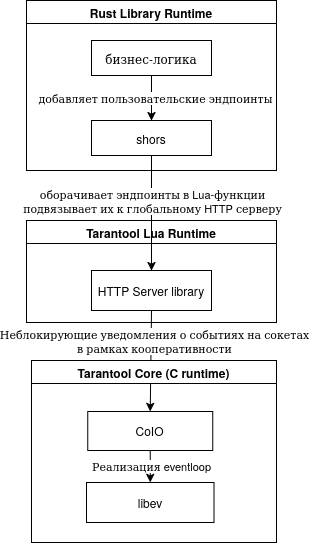
\includegraphics{existing_architecture}
\end{figure}


Преимуществом такого решения с точки зрения команды Picodata является простота реализации и поддержки - shors является небольшой библиотекой, не требующей особого ухода.
При появлении новых требований - например, интеграции генератора OpenAPI-схем, достаточно небольших включений.

Недостатком является лишний слой во взаимодействии с примитивами Tarantool - по сути для реализации высокоуровневого фреймворка shors используется другой высокоуровневый фреймворк - Lua HTTP-сервер.
В результате страдает производительность.

\section{Анализ акторных групп}\label{sec:analyze_actors}

Для формирования концепции будущего решения и его дальнейшей реализации критически необходимо изучить акторные группы существующего решения и сформировать их схематическое представление - диаграмму прецедентов.
Без этого можно упустить некоторые важные потребности пользователей, не включив их в архитектуру продукта.

Компания Picodata имеет ряд продуктов, которые используют Tarantool и фреймворк cartridge, и с очень малой вероятностью будут переделаны на полноценное использование СУБД Picodata.
Такие клиенты используют текущее решение - фреймворк shors, для реализации HTTP-интерфейса.
Компания Picodata не видит ценности в улучшении производительности HTTP-API для этих продуктов, поскольку в них нужные цели по SLA достигнуты.
Соответственно, эта акторная группа исключается из рассмотрения - клиенты будут продолжать использовать фреймворк “shors”.

Активной акторной группой являются клиенты, полноценно использующие СУБД Picodata - авторы плагинов.
На данный момент они используют “shors” для реализации HTTP-API: на новом фреймворке они хотят  аналогичную функциональность: возможность создания API-эндпоинтов с пользовательской логикой, в будущем - возможность генерации OpenAPI-схемы.

Схожей и релевантной акторной группой являются разработчики СУБД Picodata: улучшенное решение необходимо для использования внутри самой СУБД Picodata.
Сейчас СУБД Picodata представляет HTTP-API для административных целей, включая эндпоинт для сбора метрик.

В результате формируется диаграмма прецедентов, показанная на рисунке 1.3.
Наследование акторной группы пользователя остальных групп показывает, что для конечного фреймворка пользователи равнозначны.
Однако наличие двух акторных групп - важный аспект, поскольку демонстрирует присутствие нескольких потоков интересующих дополнений.

\begin{figure}[!h]
	\caption*{Рисунок 1.3 - Диаграмма прецедентов решения}\label{fig3}
	\centering
	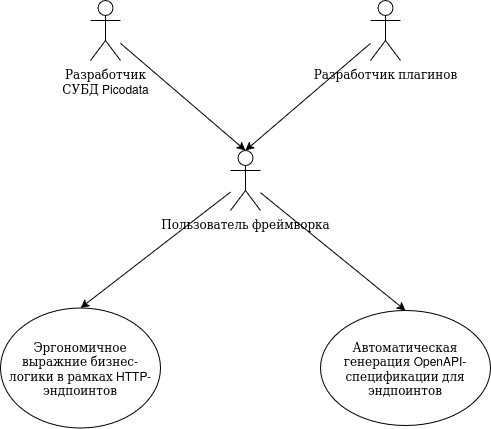
\includegraphics{actor_groups}
\end{figure}

\section{Формирование функциональных и нефункциональных требований}\label{sec:requirements}

В результате уже приведенного анализа и коммуникации с разработчиками СУБД Picodata можно выделить следующие нефункциональные требования:

\begin{enumerate}[label=\arabic*.]
	\item фреймворк должен быть в легком доступе для всех акторов - в идеале, будучи Rust-библиотекой, он должен быть представлен в публичном реестре “crates.io”;
	\item фреймворк должен предоставлять качественные абстракции: детали реализации и особенности транспорта Tarantool CoIO должны быть скрыты;
	\item фреймворк должен быть открытым ПО: HTTP-сервер - обширная тема, и возможность легкого содействия поможет привлечь сторонних разработчиков;
	\item фреймворк должен просто интегрироваться с библиотекой SDK плагинов: например, посредством реэкспорта.
\end{enumerate}

В результате изучения текущих решений с технической точки зрения и опроса акторов были выделены следующие функциональные требования:

\begin{enumerate}[label=\arabic*.]
	\item фреймворк должен предоставлять функционал пользовательской маршрутизации и обработки запросов;
	\item должна быть реализована поддержка основных HTTP-методов (GET, POST, PUT, DELETE и пр.);
	\item должна быть возможность создать эндпоинты с возможностью использования параметров запроса, группировки по тэгам;
	\item фреймворк должен просто интегрироваться с библиотекой SDK плагинов: например, посредством реэкспорта;
	\item необходима возможность реализовать middleware для предварительной и последующей обработки запросов: включая пользовательские и встроенные - для, например, логирования и обработки ошибок;
	\item фреймворк должен интегрироваться с I/O-системой Tarantool. Ожидание данных и ответ на них должны быть неблокирующими и не приводить к остановке транзакционного потока.
\end{enumerate}

\section{Листинги}

В работах студентов кафедры <<Компьютерные технологии>> часто встречаются листинги. Листинги бывают
двух основных видов~--- исходный код и псевдокод. Первый оформляется с помощью окружения \texttt{lstlisting}
из пакета \texttt{listings}, который уже включается в стилевике и немного настроен. Пример Hello World на Java
приведен на листинге~\ref{lst1}. Пример большого листинга~--- в приложении (листинг~\ref{lstX}).

\begin{lstlisting}[float=!h,caption={Пример исходного кода на Java},label={lst1}]
public class HelloWorld {
    public static void main(String[] args) {
        System.out.println("Hello, world!");
    }
}
\end{lstlisting}

Псевдокод можно оформлять с помощью разных пакетов. В данном стилевике включается пакет \texttt{algorithmicx}.
Сам по себе он не генерирует флоатов, поэтому для них используется пакет \texttt{algorithm}.
Пример их совместного использования приведен на листинге~\ref{lst2}.

\begin{algorithm}[!h]
	\caption{Пример псевдокода}\label{lst2}
	\begin{algorithmic}
		\Function{IsPrime}{$N$}
		\For{$t \gets [2; \lfloor\sqrt{N}\rfloor]$}
		\If{$N \bmod t = 0$}
		\State\Return \textsc{false}
		\EndIf
		\EndFor
		\State\Return \textsc{true}
		\EndFunction
	\end{algorithmic}
\end{algorithm}

Наконец, листинги из \texttt{listings} тоже можно подвешивать с помощью \texttt{algorithm},
пример на листинге~\ref{lst3}.

\begin{algorithm}[!h]
	\caption{Исходный код и флоат \texttt{algorithm}}\label{lst3}
	\begin{lstlisting}
public class HelloWorld {
    public static void main(String[] args) {
        System.out.println("Hello, world!");
    }
}
\end{lstlisting}
\end{algorithm}

\chapter{Проверка сквозной нумерации}

Листинг~\ref{lst4} должен иметь номер 4.

\begin{algorithm}[!h]
	\caption{Исходный код и флоат \texttt{algorithm}}\label{lst4}
	\begin{lstlisting}
public class HelloWorld {
    public static void main(String[] args) {
        System.out.println("Hello, world!");
    }
}
\end{lstlisting}
\end{algorithm}

Таблица~\ref{tab3} должна иметь номер 3.

\begin{table}[!h]
	\caption{Таблица умножения с помощью \texttt{tabularx} (фрагмент)}\label{tab3}
	\centering
	\begin{tabularx}{\textwidth}{|*{18}{>{\centering\arraybackslash}X|}}\hline
		-- & 1 & 2 & 3  & 4  & 5  & 6  & 7  & 8  & 9  & 10 & 11 & 12 & 13 & 14 & 15 & 16 & 17 \\\hline
		1  & 1 & 2 & 3  & 4  & 5  & 6  & 7  & 8  & 9  & 10 & 11 & 12 & 13 & 14 & 15 & 16 & 17 \\\hline
		2  & 2 & 4 & 6  & 8  & 10 & 12 & 14 & 16 & 18 & 20 & 22 & 24 & 26 & 28 & 30 & 32 & 34 \\\hline
		3  & 3 & 6 & 9  & 12 & 15 & 18 & 21 & 24 & 27 & 30 & 33 & 36 & 39 & 42 & 45 & 48 & 51 \\\hline
		4  & 4 & 8 & 12 & 16 & 20 & 24 & 28 & 32 & 36 & 40 & 44 & 48 & 52 & 56 & 60 & 64 & 68 \\\hline
	\end{tabularx}
\end{table}

\chapterconclusion

В конце каждой главы желательно делать выводы. Вывод по данной главе~--- нумерация работает корректно, ура!

%% Макрос для заключения. Совместим со старым стилевиком.
\startconclusionpage

В данном разделе размещается заключение.

\printmainbibliography

%% После этой команды chapter будет генерировать приложения, нумерованные русскими буквами.
%% \startappendices из старого стилевика будет делать то же самое
\appendix

\chapter{Пример приложения}\label{sec:app:1}

В приложениях рисунки, таблицы и другие подобные элементы нумеруются по приложениям с соответствующим префиксом. Проверим это.

Листинг~\ref{lst4:apx} должен иметь номер А.1.

\begin{algorithm}[!h]
	\caption{Исходный код и флоат \texttt{algorithm}}\label{lst4:apx}
	\begin{lstlisting}
public class HelloWorld {
    public static void main(String[] args) {
        System.out.println("Hello, world!");
    }
}
\end{lstlisting}
\end{algorithm}

Рисунок~\ref{fig2:apx} должен иметь номер A.1.

\begin{figure}[!h]
	\caption{Пример рисунка}\label{fig2:apx}
	\centering
	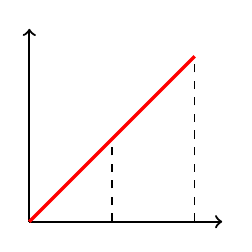
\begin{tikzpicture}[scale=0.7]
		\draw[thick,->] (0,0)--(3.5,0);
		\draw[thick,->] (0,0)--(0,3.5);
		\draw[very thick, red] (0,0)--(3,3);
		\draw[dashed] (3,0)--(3,3);
		\draw[dashed] (1.5,0)--(1.5,1.5);
	\end{tikzpicture}
\end{figure}

Таблица~\ref{tab3:apx} должна иметь номер A.1.

\begin{table}[!h]
	\caption{Таблица умножения с помощью \texttt{tabularx} (фрагмент)}\label{tab3:apx}
	\centering
	\begin{tabularx}{\textwidth}{|*{18}{>{\centering\arraybackslash}X|}}\hline
		-- & 1 & 2 & 3  & 4  & 5  & 6  & 7  & 8  & 9  & 10 & 11 & 12 & 13 & 14 & 15 & 16 & 17 \\\hline
		1  & 1 & 2 & 3  & 4  & 5  & 6  & 7  & 8  & 9  & 10 & 11 & 12 & 13 & 14 & 15 & 16 & 17 \\\hline
		2  & 2 & 4 & 6  & 8  & 10 & 12 & 14 & 16 & 18 & 20 & 22 & 24 & 26 & 28 & 30 & 32 & 34 \\\hline
		3  & 3 & 6 & 9  & 12 & 15 & 18 & 21 & 24 & 27 & 30 & 33 & 36 & 39 & 42 & 45 & 48 & 51 \\\hline
		4  & 4 & 8 & 12 & 16 & 20 & 24 & 28 & 32 & 36 & 40 & 44 & 48 & 52 & 56 & 60 & 64 & 68 \\\hline
	\end{tabularx}
\end{table}

Заодно проверим нумерованные и ненумерованные перечисления. Ненумерованные:
\begin{itemize}
	\item пункт А;
	\item пункт Б;
	\item пункт В.
\end{itemize}

Нумерованные списки нескольких уровней:
\begin{enumerate}
	\item первый элемент;
	\item второй элемент с подэлементами:
	      \begin{enumerate}
		      \item первый подэлемент;
		      \item второй подэлемент;
		      \item третий подэлемент.
	      \end{enumerate}
	\item третий элемент;
	\item четвертый элемент;
	\item пятый элемент;
	\item шестой элемент;
	\item седьмой элемент;
	\item восьмой элемент;
	\item девятый элемент;
	\item десятый элемент.
\end{enumerate}

\chapter{Еще один пример приложения с неимоверно длиннющим названием для тестирования переносов}\label{sec:app:2}

Проверим на примере таблиц, что нумерация в приложениях~--- по приложениям.
Таблица~\ref{tab3:apx2} должна иметь номер Б.1.

\begin{table}[!h]
	\caption{Таблица умножения с помощью \texttt{tabularx} (фрагмент)}\label{tab3:apx2}
	\centering
	\begin{tabularx}{\textwidth}{|*{18}{>{\centering\arraybackslash}X|}}\hline
		-- & 1 & 2 & 3  & 4  & 5  & 6  & 7  & 8  & 9  & 10 & 11 & 12 & 13 & 14 & 15 & 16 & 17 \\\hline
		1  & 1 & 2 & 3  & 4  & 5  & 6  & 7  & 8  & 9  & 10 & 11 & 12 & 13 & 14 & 15 & 16 & 17 \\\hline
		2  & 2 & 4 & 6  & 8  & 10 & 12 & 14 & 16 & 18 & 20 & 22 & 24 & 26 & 28 & 30 & 32 & 34 \\\hline
		3  & 3 & 6 & 9  & 12 & 15 & 18 & 21 & 24 & 27 & 30 & 33 & 36 & 39 & 42 & 45 & 48 & 51 \\\hline
		4  & 4 & 8 & 12 & 16 & 20 & 24 & 28 & 32 & 36 & 40 & 44 & 48 & 52 & 56 & 60 & 64 & 68 \\\hline
	\end{tabularx}
\end{table}

\chapter{Пример огромного листинга}

\begin{lstlisting}[caption={Пример большого листинга},label={lstX}]
import java.util.*;

public class Example {
    static int[] restoreOutgoing(int[] g, int[] outgoing,
                                 int vertex, int mask) {
        int[] rv = new int[1 + Integer.bitCount(mask)];
        int n = g.length;
        int current = rv.length - 1;
        while (true) {
            rv[current] = vertex;
            if (current == 0) {
                if (vertex != 0) {
                    throw new AssertionError();
                }
                return rv;
            }
            mask ^= 1 << (vertex - 1);
            int prevMask = outgoing[mask] & g[vertex];
            if (prevMask == 0) {
                throw new AssertionError();
            }
            vertex = Integer.numberOfTrailingZeros(prevMask);
            --current;
        }
    }

    static int[] restoreIncoming(int[] g, int[] incoming,
                                 int vertex, int mask) {
        int[] rv = new int[1 + Integer.bitCount(mask)];
        int n = g.length;
        int current = 0;
        while (true) {
            rv[current] = vertex;
            if (current == rv.length - 1) {
                if (vertex != 0) {
                    throw new AssertionError();
                }
                return rv;
            }
            mask ^= 1 << (vertex - 1);
            int nextMask = incoming[mask] & g[vertex];
            if (nextMask == 0) {
                throw new AssertionError();
            }
            vertex = Integer.numberOfTrailingZeros(nextMask);
            ++current;
        }
    }
}
\end{lstlisting}

\end{document}
